\documentclass[10pt,pdf,hyperref={unicode}]{beamer}

\mode<presentation>
{
	\usetheme{boxes}
	\beamertemplatenavigationsymbolsempty
	
	\setbeamertemplate{footline}[page number]
	\setbeamersize{text margin left=1em, text margin right=0.5em}
}

\usepackage[utf8]{inputenc}
\usepackage[english, russian]{babel}
\usepackage[normalem]{ulem}
\usepackage{bm}
\usepackage{multirow}
\usepackage{ragged2e}
\usepackage{indentfirst}
\usepackage{multicol}
\usepackage{subfig}
\usepackage{amsmath,amssymb}
\usepackage{dsfont}
\usepackage{enumerate}
\usepackage{mathtools}
\usepackage{comment}
\usepackage{tabularx, tabulary, multicol}
\usepackage[all]{xy}

\newcommand{\bz}{\mathbf{z}}
\newcommand{\bx}{\mathbf{x}}
\newcommand{\by}{\mathbf{y}}
\newcommand{\bv}{\mathbf{v}}
\newcommand{\bw}{\mathbf{w}}
\newcommand{\ba}{\mathbf{a}}
\newcommand{\bb}{\mathbf{b}}
\newcommand{\bff}{\mathbf{f}}
\newcommand{\bh}{\mathbf{h}}
\newcommand{\bg}{\mathbf{g}}
\newcommand{\bl}{\mathbf{l}}
\newcommand{\bp}{\mathbf{p}}
\newcommand{\bq}{\mathbf{q}}
\newcommand{\bs}{\mathbf{s}}
\newcommand{\bt}{\mathbf{t}}
\newcommand{\bu}{\mathbf{u}}
\newcommand{\bT}{\mathbf{T}}
\newcommand{\bX}{\mathbf{X}}
\newcommand{\bZ}{\mathbf{Z}}
\newcommand{\bS}{\mathbf{S}}
\newcommand{\bH}{\mathbf{H}}
\newcommand{\bW}{\mathbf{W}}
\newcommand{\bY}{\mathbf{Y}}
\newcommand{\bU}{\mathbf{U}}
\newcommand{\bQ}{\mathbf{Q}}
\newcommand{\bP}{\mathbf{P}}
\newcommand{\bA}{\mathbf{A}}
\newcommand{\bB}{\mathbf{B}}
\newcommand{\bC}{\mathbf{C}}
\newcommand{\bE}{\mathbf{E}}
\newcommand{\bF}{\mathbf{F}}
\newcommand{\bsigma}{\boldsymbol{\sigma}}
\newcommand{\bomega}{\boldsymbol{\omega}}
\newcommand{\btheta}{\boldsymbol{\theta}}
\newcommand{\bgamma}{\boldsymbol{\gamma}}
\newcommand{\bdelta}{\boldsymbol{\delta}}
\newcommand{\bPsi}{\boldsymbol{\Psi}}
\newcommand{\bpsi}{\boldsymbol{\psi}}
\newcommand{\bxi}{\boldsymbol{\xi}}
\newcommand{\bmu}{\boldsymbol{\mu}}
\newcommand{\bchi}{\boldsymbol{\chi}}
\newcommand{\bzeta}{\boldsymbol{\zeta}}
\newcommand{\blambda}{\boldsymbol{\lambda}}
\newcommand{\beps}{\boldsymbol{\varepsilon}}
\newcommand{\bZeta}{\boldsymbol{Z}}
% mathcal
\newcommand{\cX}{\mathcal{X}}
\newcommand{\cY}{\mathcal{Y}}
\newcommand{\cW}{\mathcal{W}}
\newcommand{\cL}{\mathcal{L}}

\newcommand{\dH}{\mathds{H}}
\newcommand{\dR}{\mathds{R}}
% transpose
\newcommand{\T}{^{\mathsf{T}}}

% command to strike out text
\newcommand{\stkout}[1]{\ifmmode\text{\sout{\ensuremath{#1}}}\else\sout{#1}\fi}

% limited alertblock
\newenvironment<>{varblock}[2][.9\textwidth]{%
	\setlength{\textwidth}{#1}
	\begin{actionenv}#3%
		\def\insertblocktitle{#2}%
		\par%
		\usebeamertemplate{block begin}}
	{\par%
		\usebeamertemplate{block end}%
\end{actionenv}}

\renewcommand{\epsilon}{\ensuremath{\varepsilon}}
\renewcommand{\phi}{\ensuremath{\varphi}}
\renewcommand{\kappa}{\ensuremath{\varkappa}}
\renewcommand{\le}{\ensuremath{\leqslant}}
\renewcommand{\leq}{\ensuremath{\leqslant}}
\renewcommand{\ge}{\ensuremath{\geqslant}}
\renewcommand{\geq}{\ensuremath{\geqslant}}
\renewcommand{\emptyset}{\varnothing}

\usepackage{tikz}
\usetikzlibrary{positioning,arrows}

\tikzstyle{name} = [parameters]
\definecolor{name}{rgb}{0.5,0.5,0.5}

\usepackage{caption}
\captionsetup{skip=0pt,belowskip=0pt}

\newtheorem{rustheorem}{Теорема}
\newtheorem{russtatement}{Утверждение}
\newtheorem{rusdefinition}{Определение}

% colors
\definecolor{darkgreen}{rgb}{0.0, 0.2, 0.13}
\definecolor{darkcyan}{rgb}{0.0, 0.55, 0.55}

\AtBeginEnvironment{figure}{\setcounter{subfigure}{0}}

\captionsetup[subfloat]{labelformat=empty}
\addto\captionsrussian{\renewcommand{\figurename}{}}
\graphicspath{{../figures/}}

%----------------------------------------------------------------------------------------------------------

\title[Заголовок]{Состязательные атаки на нейронные сети для работы
	с временными рядами}
\author{Владимиров Э.А.}

\institute[]{Московский физико-технический институт}
\date{\footnotesize
	\par\smallskip\emph{Научный руководитель:} к.~ф.-м.~н. А.\,А.~Зайцев
	\par\bigskip\small 2023}

%---------------------------------------------------------------------------------------------------------
\begin{document}
	
	\begin{frame}
		\titlepage
	\end{frame}
	
	%----------------------------------------------------------------------------------------------------------
	\begin{frame}{Состязательные атаки и временные ряды}
		\begin{alertblock}{Проблема}
			Состязательные атаки в области временных рядов могут быть легко обнаружены
		\end{alertblock}
		
		\begin{alertblock}{Задача}
			Предложить свой метод состязательной атаки, которую тяжело задетектировать
		\end{alertblock}
		
		\begin{alertblock}{Решение}
			Использование регуляризаторов, которые "маскируют" атаку
		\end{alertblock}
	\end{frame}
	
	%---------------------------------------------------------------------------------------------------------
	\begin{frame}{Состязательные атаки в разных доменах}
		\begin{multicols}{2}
			\begin{figure}[bhtp]
				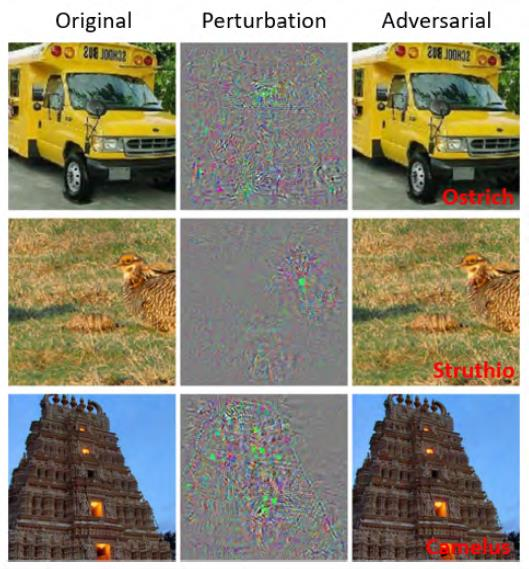
\includegraphics[width=0.4\textwidth]{attack-on-images}
				\caption{Image domain}
			\end{figure}
			
			\begin{figure}[bhtp]
				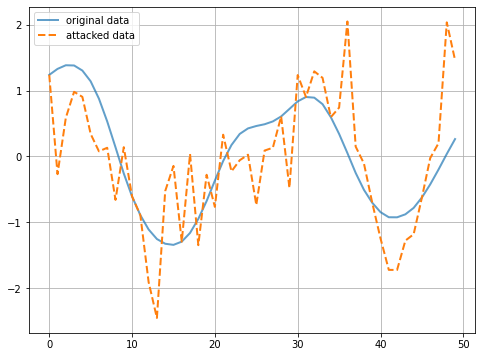
\includegraphics[width=0.47\textwidth]{attack-on-time-series}
				\caption{Time series domain}
			\end{figure}
		\end{multicols}
	
		\begin{block}{Проблема}
			Состязательные атаки в домене временных рядов легко обнаружить человеческим взглядом или специальными моделями
		\end{block}
	\end{frame}
	
	%--------------------------------------------------------------------------------------------------------
	\begin{frame}{Статьи по теме}
		\begin{enumerate}
			\item Sokerin P., Zaytsev A  Adversarial attacks on neural networks for sequential data
			\item Vivek B. S., Babu R. V. Regularizers for single-step adversarial training 
			chaos from measurement error in time series.
			\item Pialla G. et al. Time series adversarial attacks: an investigation of smooth perturbations and defense approaches 
		\end{enumerate}
	\end{frame}

	
	\begin{frame}{Постановка задачи}
		Имеется обученный классификатор временных рядов $\bff_\theta: \dR^{E \times T} \longrightarrow [0, 1]$
		
		Имеется обученный дискриминатор, определяющий искажённость данных: $\bg_\kappa: \dR^{E \times T} \longrightarrow [0, 1]$
		
		Цель: найти преобразование данных $\varphi: \dR^{E \times T} \longrightarrow \dR^{E \times T}$, оптимальное с точки зрения
		
		\begin{itemize}
			\item эффективности: $\text{effectiveness} = \dfrac{1}{n}\sum\limits_{i=1}^n [ \bff_\theta(\bx^i) = y^i] - \dfrac{1}{n}\sum\limits_{i=1}^n [ \bff_\theta(\varphi(\bx^i)) = y^i]$
			
			\item скрытности: $\text{concealability} = 1 - \dfrac{1}{n}\sum\limits_{i=1}^n \bg_\kappa(\varphi(\bx^{(i)}))$
		\end{itemize}
	\end{frame}
	
	%---------------------------------------------------------------------------------------------------------
	\begin{frame}{IFGSM и его модификация}
		\begin{multicols}{2}
			\begin{align*}
				\text{Iterative Fast Gradient Sign Method} \\
				\bx_{t+1} = \bx_t + \epsilon \cdot sign \bigl( \nabla_x \cL (\bff_\theta(\bx_t), \by) \bigr)
			\end{align*}
		
			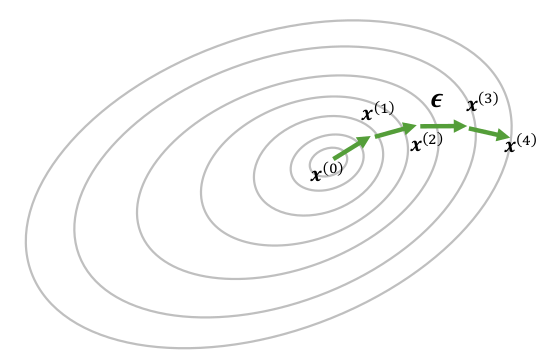
\includegraphics[width=0.45\textwidth]{loss-space}
		\end{multicols}
	
		\begin{block}{Предлагаемое улучшение}
			\begin{align*}
				\bh_{t+1} &= \bx_t + \epsilon \cdot sign \bigl( \nabla_x \cL (\bff_\theta(\bx_t), \by) \bigr) \\
				\Delta_{t+1} &= || \bx_0 - \bh_{t+1} || \\
				\bx_{t+1} &= \bx_t + \epsilon_{\max} clip \bigl( \nabla_x \cL (\bff_\theta(\bx_t), \by), -\exp(-\Delta_{t+1}^2), \exp(-\Delta_{t+1}^2) \bigr)
			\end{align*}
		\end{block}
	\end{frame}
	%----------------------------------------------------------------------------------------------------------
	\begin{frame}{Вычислительный эксперимент}
		\begin{varblock}{Цель}
			Сравнение состязательных атак для разных датасетов и архитектур нейросети
		\end{varblock}
		
%		\textbf{Модели}: LSTM, TS2Vec, S4
		
%		\textbf{Датасеты}: FordA, Coffee
		
		\begin{table}[bhtp]
			\begin{tabular}{|l|l|l|l|}
				\hline
				\multicolumn{1}{|c|}{\multirow{2}{*}{Attack}} & \multicolumn{1}{c|}{Dataset} & \multicolumn{1}{c|}{Coffee} & FordA \\ \cline{2-4} 
				\multicolumn{1}{|c|}{}                        & Target model                 & TS2Vec & TS2Vec        \\ \hline
				\multirow{2}{*}{Vanilla IFGSM}                & Effectiveness                & \textbf{1.00}               & \textbf{1.00} \\ \cline{2-4} 
				& Concealability               & 0.08                        & 0.28          \\ \hline
				\multirow{2}{*}{Modified IFGSM}               & Effectiveness                & \textbf{1.00}               & 0.99          \\ \cline{2-4} 
				& Concealability               & \textbf{0.97}               & \textbf{0.92} \\ \hline
			\end{tabular}
		\end{table}
		
	\end{frame}
	
	%----------------------------------------------------------------------------------------------------------
	\begin{frame}{Визуализация состязательных атак}
		\begin{multicols}{2}
			\begin{figure}[bhtp]
				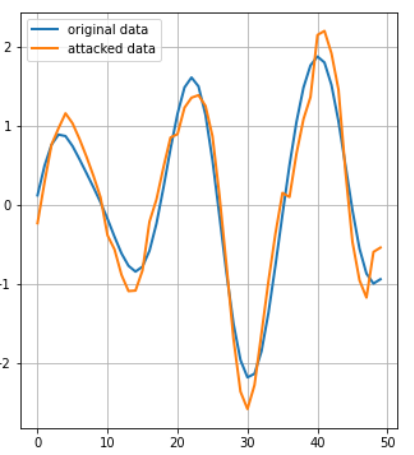
\includegraphics[width=0.45\textwidth]{vanilla-ifgsm}
				\caption{Vanilla IFGSM}
			\end{figure}
			
			\begin{figure}[bhtp]
				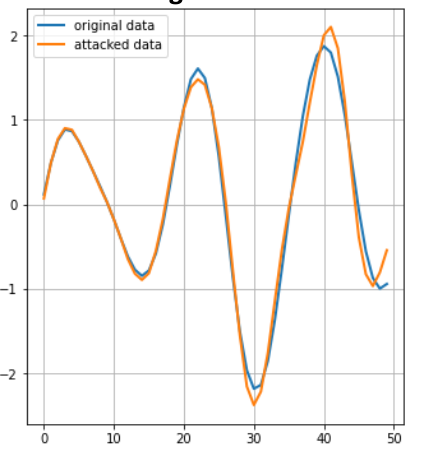
\includegraphics[width=0.45\textwidth]{modified-ifgsm}
				\caption{Modified IFGSM}
			\end{figure}
		\end{multicols}
	\end{frame}
	
	%----------------------------------------------------------------------------------------------------------
	\begin{frame}{Заключение}
		\begin{enumerate}
			
			\item Предложен новый способ состязательной атаки
			
			\item Проведён вычислительный эксперимент на нескольких датасетах
			
		\end{enumerate}
	\end{frame}
	
\end{document} 